\documentclass[10pt]{beamer}

\usepackage{fontspec}
\setmainfont{Ubuntu}[]
\setsansfont{Ubuntu}[]
\setmonofont{Ubuntu Mono}[]

\usepackage{graphicx}
\graphicspath{ {../img/} }

\beamertemplatenavigationsymbolsempty

\title{Свойства BEAM}

\begin{document}

\begin{frame}
  \frametitle{Erlang Virtual Machine}
  Эликсир и Эрланг объединяет виртуальная машина EVM (Erlang~Virtual~Machine),
  \par \bigskip
  которую обычно называют \textbf{BEAM} (Bogdan's~Erlang~Abstract~Machine).
\end{frame}

\begin{frame}
  \frametitle{Erlang Virtual Machine}
  Операционная система в миниатюре:
  \begin{itemize}
  \item планировщик процессов,
  \item управление памятью,
  \item ввод-вывод,
  \item сетевой стек,
  \item и др.
  \end{itemize}
\end{frame}

\begin{frame}
  \frametitle{Erlang Virtual Machine}
  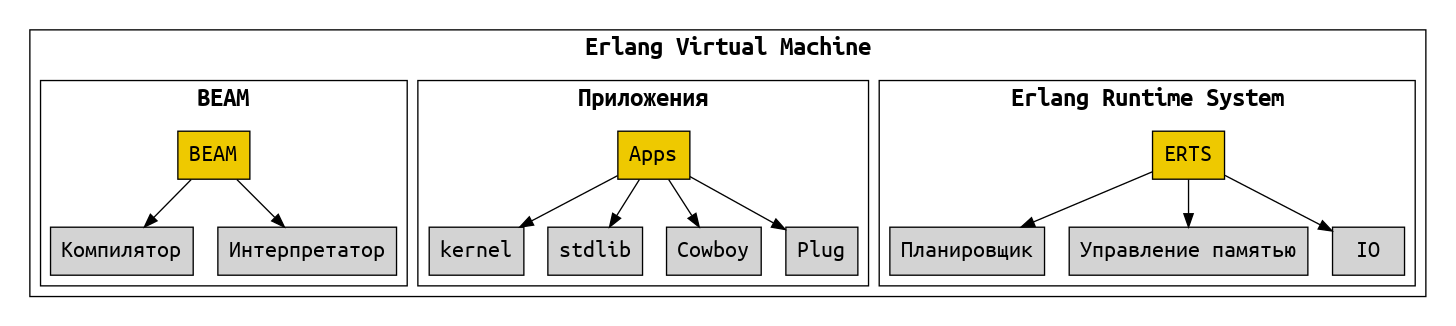
\includegraphics[scale=0.2]{evm}
\end{frame}

\begin{frame}
  \frametitle{Erlang Virtual Machine}
  Основные свойства машины:
  \begin{itemize}
  \item Многопоточность (Concurrency);
  \item Устойчивость к ошибкам (Fault Tolerance);
  \item Поддержка распределенных систем (Distribution);
  \item Горячее обновление кода (Hot Code Upgrade).
  \end{itemize}
\end{frame}

\begin{frame}
  \frametitle{Erlang Virual Machine}
  Еще несколько свойств:
  \begin{itemize}
  \item Симметричная многопроцессорность (Symmetric~Multiprocessing);
  \item Модель акторов (Actor Model);
  \item Система реального времени (Soft Real Time);
  \item Сборщик мусора (Garbage Collector);
  \item Интерактивная консоль (Erlang/Elixir Shell);
  \item Трассировка (Tracing).
  \end{itemize}
\end{frame}

\begin{frame}
  \frametitle{Многопоточность}
  Процессы (thread) и планировщики (scheduler), независимые~от~ОС.
  \par \bigskip
  Процессы легковесные, их можно создавать десятки и~сотни~тысяч.
  \par \bigskip
\end{frame}
  
\begin{frame}
  \frametitle{Многопоточность}
  Каждый процесс имеет свою изолированную память, разделяемой памяти (shared memory) нет.
  \par \bigskip
  Процессы изолированы, блокировка или падение одного процесса не влияет на работу остальных.
  \par \bigskip
  Данные передаются отправкой сообщений (message passing).
\end{frame}

\begin{frame}
  \frametitle{Многопоточность}
  BEAM способна запускать до \textbf{134,217,727} ($2^{27}$) процессов.
  \par \bigskip
  Запуск нового процесса занимает \textbf{3-5 микросекунд}.
  \par \bigskip
  На старте процесс резервирует \textbf{2696 байт} памяти, включая стек, кучу~и~метаданные.
\end{frame}


\begin{frame}
  \frametitle{Многопоточность}
  Отдельный планировщик на каждом ядре CPU.
  \par \bigskip
  Балансируют нагрузку, передавая процессы друг другу.
\end{frame}

\begin{frame}
  \frametitle{Устойчивость к ошибкам}
  Исключения не основной способ обработки ошибок.
  \par \bigskip
  Основной способ -- это механизм мониторинга одних~процессов~другими.
  \par \bigskip
  \textbf{supervisor} (наблюдатель) и \textbf{worker} (рабочий процесс).
\end{frame}

\begin{frame}
  \frametitle{Устойчивость к ошибкам}
  Супервизоры наблюдают за рабочими процессами и~друг~за~другом.
  \par \bigskip
  Организованы в дерево, где узлами являются супервизоры, а~листьями~–~рабочие процессы.
\end{frame}

\begin{frame}
  \frametitle{Устойчивость к ошибкам}
  Следущий уровень устойчивости к ошибкам -- объединение узлов в кластер.
  \par \bigskip
  Если узел падает, то его функцию берет на себя другой узел.
\end{frame}


%% \begin{frame}
%%   \frametitle{}
%% \end{frame}

%% \begin{frame}
%%   \frametitle{}
%% \end{frame}

\end{document}
